\documentclass[a4j,12pt,]{jarticle}
 \usepackage{float}
 \usepackage{siunitx} %%SI単位系用
 \usepackage{amssymb, amsmath}
 \usepackage{ascmac,here,txfonts}
 \usepackage{hyperref}
 \usepackage{listings}
 \usepackage{pxjahyper}
 \usepackage[dvipdfmx]{graphicx}
 \usepackage{amssymb, amsmath}
  \usepackage{listings}
  \usepackage[dvipdfmx]{color}
 
 \lstset{
   language={Python},
   basicstyle={\ttfamily},
   identifierstyle={\small},
   commentstyle={\small\itshape},
   keywordstyle={\small\bfseries},
   ndkeywordstyle={\small},
   stringstyle={\small\ttfamily},
   frame={single},
   breaklines=true,
   columns=[l]{fullflexible},
   numbers=left,
   xrightmargin=0zw,
   xleftmargin=3zw,
   numberstyle={\scriptsize},
   stepnumber=1,
   numbersep=1zw,
   lineskip=-0.5ex,
 }
\begin{document}

{\noindent\small 第19回報告書 \hfill\today}
\begin{center}
  {\Large 133.71.106.141のElasticSearchサーバーのco2インデックスとco2\_modbusインデックス間のデータの移行について}
\end{center}
\begin{flushright}
  祖父江匠真 \\
\end{flushright}

\section{概要}
今回は, CO\textsubscript{2}データの収集を行っているラズベリーパイの一部が133.71.106.141のElasticSearchサーバーにあるco2インデックスに対してインサートを行ったことにより, co2\_modbusインデックス以外のインデックスに一部のCO\textsubscript{2}データが保存されている問題を解消したことについて報告する.

\section{データ移行手順について}

ラズベリーパイからco2インデックスに対してインサートした全てのドキュメントをローカルマシンにJSON形式でエクスポートして, 作成したPythonプログラムを実行してco2\_modbusインデックスにインサートした.

\subsection{データのエクスポート}
移行元のElasticSearchサーバーのデータのローカルマシンへのエクスポートには, elasticdump \cite{1}ライブラリを使用してJSON形式でエクスポートした.

co2インデックスに対してラズベリーパイからインサートしたデータにはJPtimeフィールドが存在しないため, JPtimeフィールドが存在しないドキュメントのみをエクスポートした.

また, エクスポートしたJSONデータを解析したところ, 最も古いutctimeフィールドの日付は2023年7月5日だった.

\subsection{データのインポート}
エクスポートしたJSONファイルを, 作成したPythonプログラムから読み込んで, Pythonのelasticsearchライブラリを用いてco2\_modbusインデックスにインサートした.

\section{データ移行が正常に行えたか確認}
図 \ref{p2}にco2インデックスの2023年7月以降のPPM値の推移をグラフにしたものを, 図 \ref{p3}にco2\_modbusインデックスの2023年7月以降のPPM値の推移をグラフにしたものを示す.

図 \ref{p2}と図 \ref{p3}より, co2インデックスのデータが正常にco2\_modbusインデックスに移行できていることが分かる.

\begin{figure}[H]
  \begin{center}
    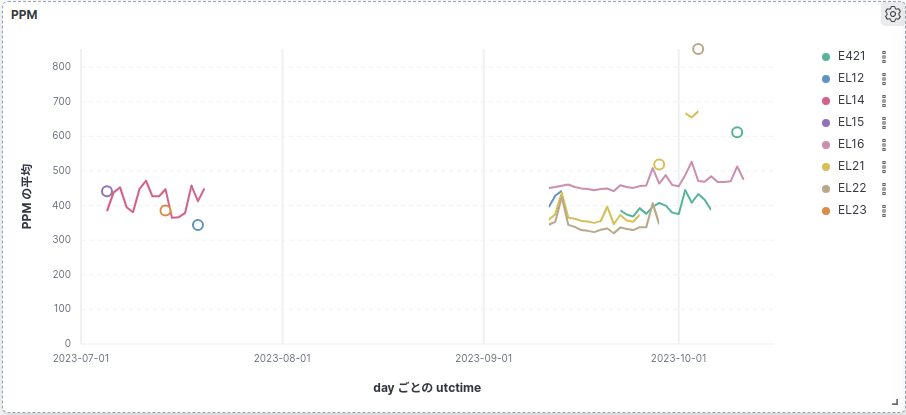
\includegraphics[width=160mm]{co2PPM.png}
    \caption{co2インデックスのPPM}
    \label{p2}
  \end{center}
\end{figure}

\begin{figure}[H]
  \begin{center}
    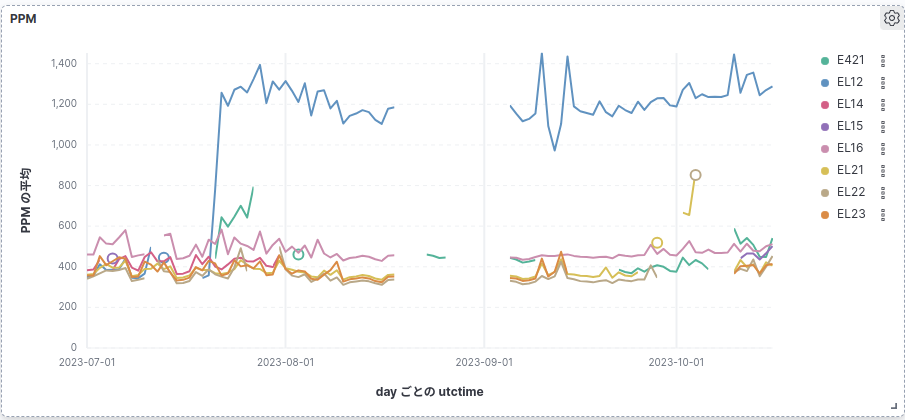
\includegraphics[width=160mm]{co2ModbusPPM.png}
    \caption{co2\_modbusインデックスのPPM}
    \label{p3}
  \end{center}
\end{figure}

次に, 図 \ref{p4}にco2インデックスの2023年7月以降のRH値の推移をグラフにしたものを, 図 \ref{p5}にco2\_modbusインデックスの2023年7月以降のRH値の推移をグラフにしたものを示す.

図 \ref{p4}と図 \ref{p5}より, co2インデックスのデータが正常にco2\_modbusインデックスに移行できていることが分かる.

\begin{figure}[H]
  \begin{center}
    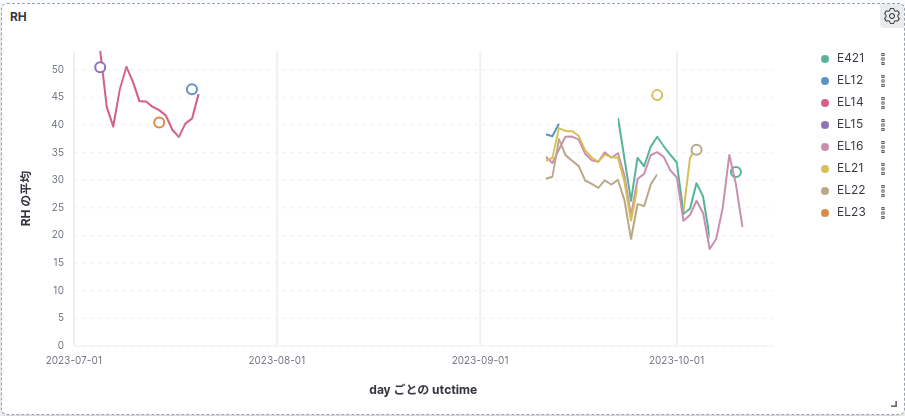
\includegraphics[width=160mm]{co2RH.png}
    \caption{co2インデックスのRH}
    \label{p4}
  \end{center}
\end{figure}

\begin{figure}[H]
  \begin{center}
    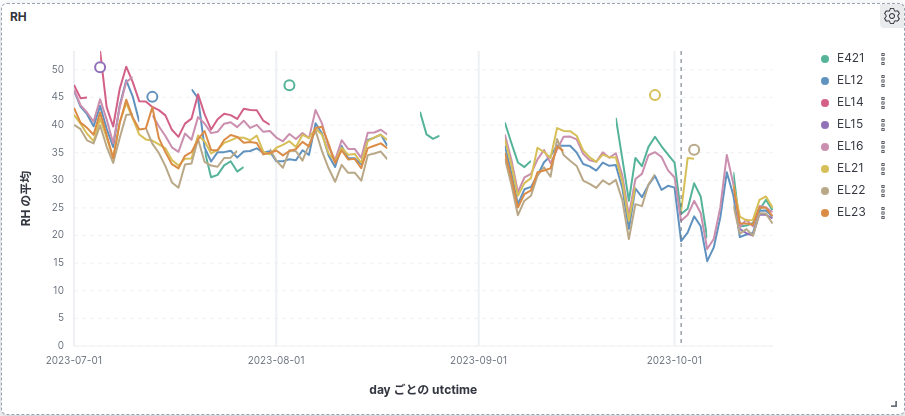
\includegraphics[width=160mm]{co2ModbusRH.png}
    \caption{co2\_modbusインデックスのRH}
    \label{p5}
  \end{center}
\end{figure}

次に, 図 \ref{p6}にco2インデックスの2023年7月以降のTEMP値の推移をグラフにしたものを, 図 \ref{p7}にco2\_modbusインデックスの2023年7月以降のTEMP値の推移をグラフにしたものを示す.

図 \ref{p6}と図 \ref{p7}より, co2インデックスのデータが正常にco2\_modbusインデックスに移行できていることが分かる.

\begin{figure}[H]
  \begin{center}
    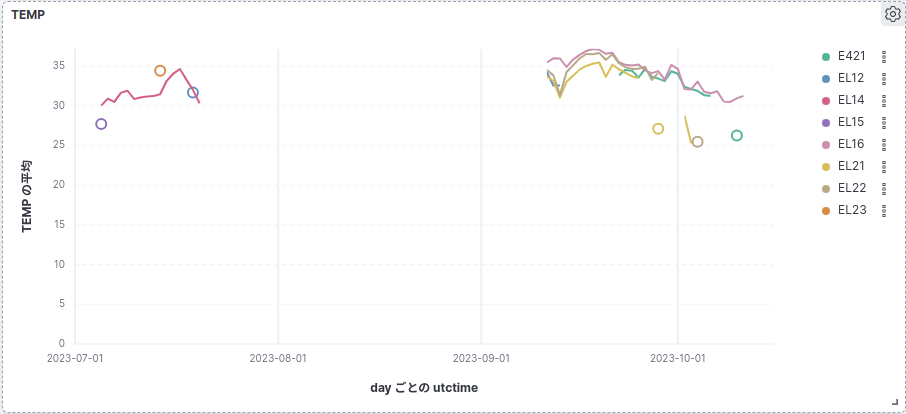
\includegraphics[width=160mm]{co2Temp.png}
    \caption{co2インデックスのTEMP}
    \label{p6}
  \end{center}
\end{figure}

\begin{figure}[H]
  \begin{center}
    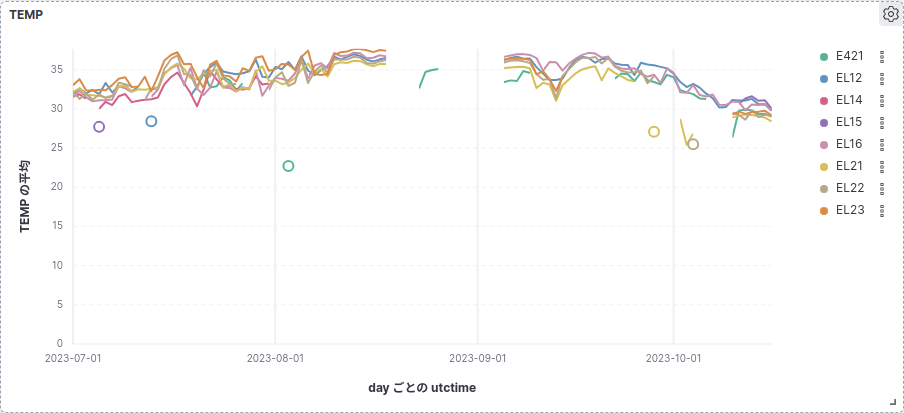
\includegraphics[width=160mm]{co2ModbusTemp.png}
    \caption{co2\_modbusインデックスのTEMP}
    \label{p7}
  \end{center}
\end{figure}

\section{まとめ}
今回は, CO\textsubscript{2}データの収集を行っているラズベリーパイの一部が133.71.106.141のElasticSearchサーバーにあるco2インデックスに対してインサートを行ったことにより, co2\_modbusインデックス以外のインデックスに一部のCO\textsubscript{2}データが保存されている問題を解消し, kibana用いてデータ移行が正しく行えたことを確認した.

次回は, リサイクル館の太陽光発電データの保存先の移行作業について報告する.

\begin{thebibliography}{5}
  \bibitem{1}Ferron H, ”ElasticDump”, https://github.com/elasticsearch-dump/elasticsearch-dump, 参照 June 19,2023.
\end{thebibliography}

\end{document}

